\begin{table*}[t]
	\caption{Comparisons with existing methods on YouTubeVOS. To save space, the year of method is not listed.}\smallskip
	
	\centering
	\resizebox{2.0\columnwidth}{!}{
		\smallskip\begin{tabular}{c|c|c|c|c|c|c|c|c|c|c }
			\hline
			&\multicolumn{3}{c|}{Fixed Square Mask}& \multicolumn{3}{c|}{Moving Square Mask}&\multicolumn{3}{c|}{Free-Form Mask}&Inference \\
			\cline{2-10} 
			&PSNR & SSIM & FID & PSNR & SSIM & FID & PSNR & SSIM & FID&Speed(fps))\\
			\hline
			Nazeri et al. &28.6446 &0.9484  &   38.2116  &	
			30.7478 & 0.9647 &  16.2739  &
			25.6693  & 0.9088 &  43.0366&22.81 \\
			\hline
			Wang et al. &27.9668 & 0.9515 &  40.7199  &	 
			31.5776	& 0.9678 &  13.8383&   
			32.1862 & 0.9626 & 19.1191 &8.1634 \\
			\hline
			
			
			Kim et al. b& 28.0846&0.9468 &  39.9377  & 
			36.8598	& 0.9728 &7.2315  &
			33.5549	& 0.9646 & 9.3797&1.2275  \\
			\hline
			Xu et al. &29.0531 & 0.9497 &  32.8860  & 
			35.9941& 0.9772 &6.3746  &
			32.6287 &0.9618  &  11.1501&0.5620 \\
			\hline
			
			\hline
			
			
			STI &28.0174 &0.9494  &  42.7164   &	
			33.8131 &  0.9705  &8.2390	& 
			30.0680& 0.9390 & 20.6358&7.6335
			\\
			\hline
			+edge input  &29.5242 &  0.9520& 36.2097   &	
			37.6630	& 0.9798 &3.5161    &	
			33.8206	&0.9659  &    6.6651& 5.2356 \\
			\hline
			
			+SAM &29.9918 &  0.9533 &  27.4198  &	
			38.2433	& 0.9807 &   2.5083  &	
			35.7783	&0.9712  &   5.8786 & 5.1546\\
			\hline
			
			
			
			
			Ours &\textbf{30.0590} &\textbf{0.9543}&   \textbf{27.2431} &
			\textbf{38.8186} & \textbf{0.9824} & \textbf{2.3455} &
			\textbf{35.9613}  & \textbf{0.9721}&  \textbf{ 5.8694} &2.5643\\
			
			\hline
			
			
		\end{tabular}
	}
	\label{tab:sem}
\end{table*}


\section{Experiments}


In order to evaluate the effect of different components in our SOVI and compare with other state-of-the-art approaches, we conduct a series of experiments on two datasets, YoutubeVOS \cite{xu2018youtube} and DAVIS \cite{davis_2017}.
%We test on two datasets, YoutubeVOS \cite{xu2018youtube} and DAVIS \cite{davis_2017}, to compare the proposed STSENet with state-of-the-art methods. %Several ablation studies are conducted to prove the effectiveness of spatial details and temporal information in video inpainting.
\subsection{Experimental Settings}
\textbf{Dataset.} 
YoutubeVOS and DAVIS are widely used for evaluation in recent video inpainting approaches.
YoutubeVOS is a large-scale dataset that contains 4,453 YouTube video clips. These videos are close to real-world scenario with 70+ common objects. 
The videos are officially split into three parts, 3,471 for training, 474 for validating, and 508 for testing. 
DAVIS dataset is for video object segmentation containing 150 video clips, among which 60 randomly sampled clips are for testing of object removal. And the rest part is used for training.
The videos are complex with occlusions, fast motion, and various objects. 

\noindent \textbf{Mask Setting.} Considering various real-world applications, we test our method on four kinds of mask settings in this paper. 
They are different in shapes and positions of the missing regions.
\begin{enumerate}
	\item Fixed square mask. The size and position of the missing square region are fixed through the whole video. 
	\item Moving square mask. The position and size of the square mask change over frames. 
	\item Free-from mask. We apply irregular mask which imitates hand-drawn masks on each frame, following \cite{liu2018partialinpainting}. 
	\item Foreground object mask. This type of masks are defined to line out the foreground objects in videos, which is used for object removal.
\end{enumerate}

	
\noindent \textbf{Implementation Details.} 
In the data preparation stage, we random sample a clip every 40 frames from each video in the datasets and resize the video frames into $256\times256$.
%
During training, we first train our ENet and FNet jointly using Adam optimizer with $\beta=(0.9, 0.999)$.
The learning rate is set to $1e-4$ for $N^E$ and $G^F$ and 1e-5 for $D^E$. Then, the STINet is trained with the learning rate of 1e-4 for $G^I$, and 4e-4 for $D^I$. Finally, the temporal ensemble module is trained with the learning rate of 1e-4.  We do not use weight decay in training.
As for the hyper-parameters, $\lambda_1=10.0,\lambda_2=\lambda_3=0.1,\lambda_4=300.0,\lambda_5=5.0$.

\noindent \textbf{Evaluation Metrics.} 
We use three commonly-used metrics to quantitatively evaluate the performance of our method. They are structural similarity index (SSIM) \cite{wang2004image}, peak signal-to-noise ratio (PSNR), and Fr{\'e}chet Inception Distance (FID) \cite{heusel2017gans}. 
Besides, the quantitative metrics can not be used in the experiments of foreground object removal, since there is no ground truth available. So we conduct a user study for video foreground object removal. 
%\cxj{Where these three metrics are used compared with object removal?}
%
%Besides, since there is no ground truth for the experiments of object removal, 




\begin{figure*}[t]
	\centering
	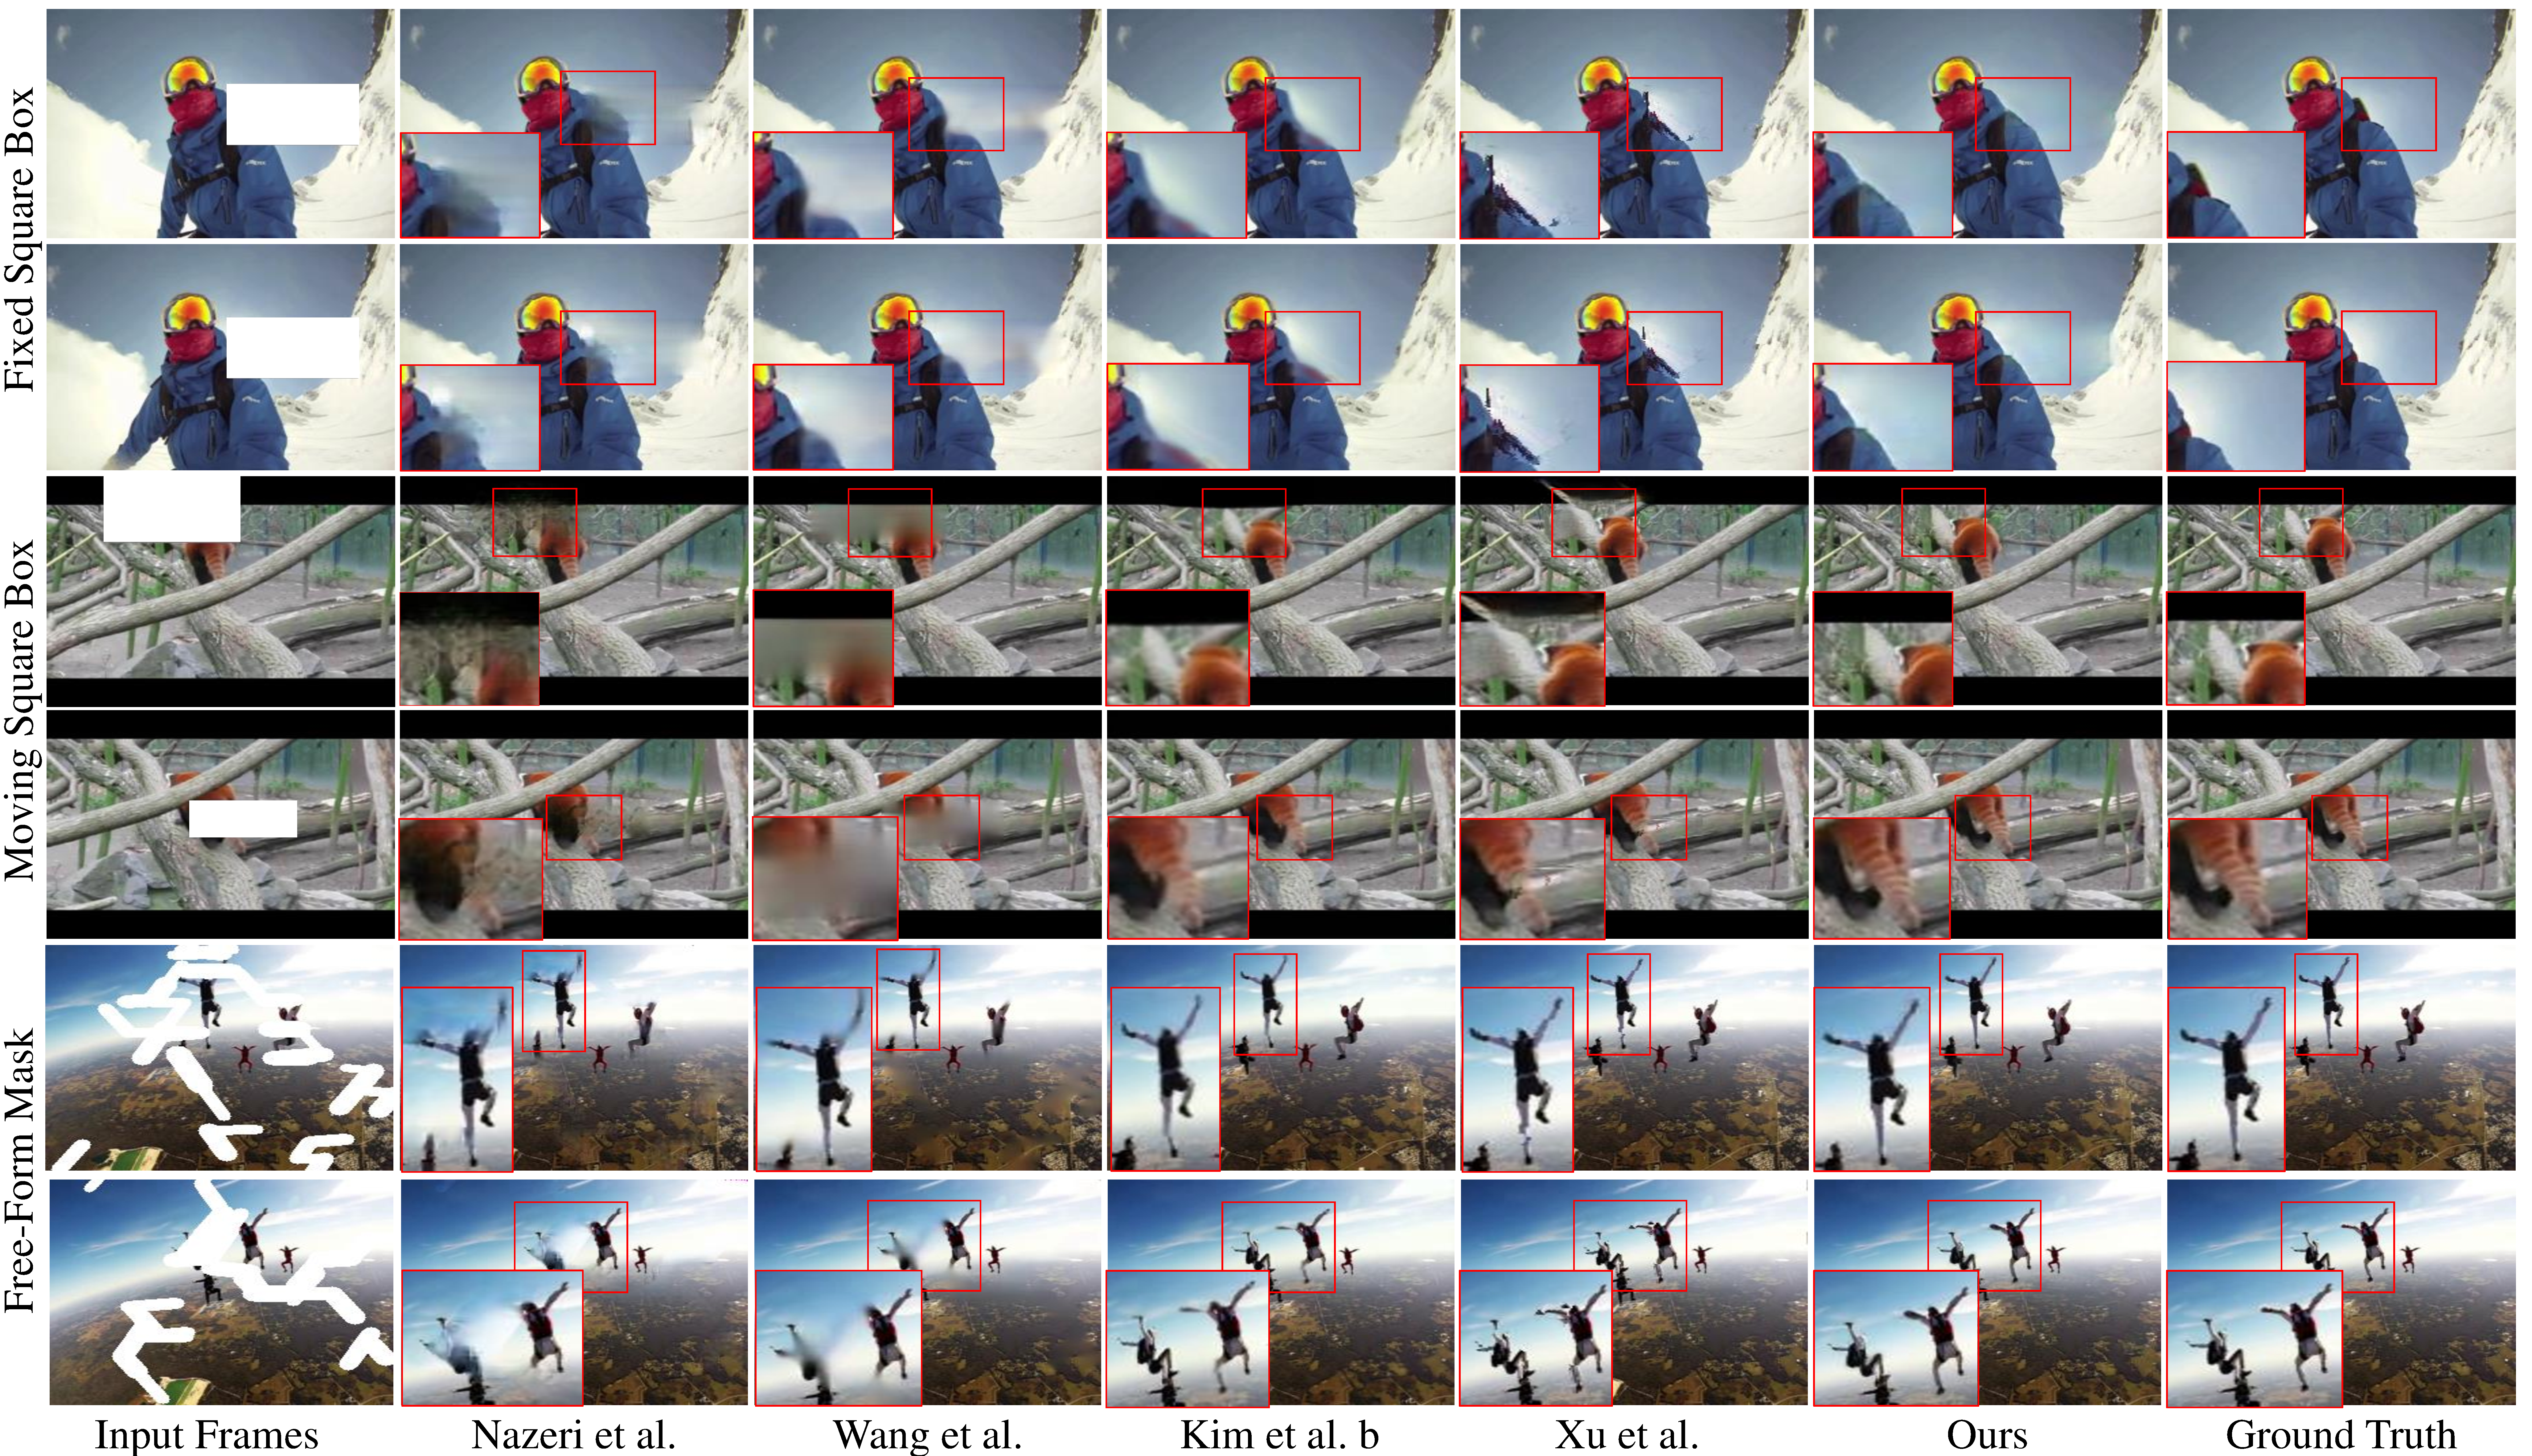
\includegraphics[scale=0.127]{viszong} % Reduce the figure size so that it is slightly narrower than the column. Don't use precise values for figure width.This setup will avoid overfull boxes. 
	\caption{Visualization for video inpainting on YouTubeVOS. Our method can produce frames with finer sturcture than existing methods. }
	\label{viszong}
\end{figure*}

\subsection{Ablation Study}
To demonstrate the effectiveness of proposed components in our method, we first conduct ablation study on YouTubeVOS. 

\subsubsection{Effect of Structure Clues in STINet.}

To evaluate the effects of structural information in video inpainting, we successively put each part related with structure to the baseline and compare the performances. We use three variants of our model: 'STI', '+edge input', and '+SAM'. 
'STI' is the baseline using only the spatio-temporal inpainting network, without either structure clues or temporal information. '+edge input' is the model that uses the predicted edge maps as input. '+SAM' is the model in which structure attention module is applied.

The quantitative results are shown in Table~\ref{tab:sem}. We can see that both the designed parts regarding structure information are beneficial to video inpainting.
As shown, the network achieves better results when edge information is utilized, comparing '+edge input' to 'STI'. It indicates that edge clues are effective guidance in video inpainting, which helps the network to predict more accurate frames.
When we further add structure attention module to the network, it can bring an extra stable improvement to the results. It demonstrates that the latent structure information of edge maps can not be fully utilized when naively used as input. SAM is effective to encode the spatial correlation between edge maps and video contents, which assists the network to learn to inpaint structure-preserved frames efficiently.
%SAM is useful for the network to 



%the superiority of SEM is evaluated by comparing its performance with the method, that replaces the attention map in Fig.~\ref{SEM} with edge map.
%The results are reported in Table~\ref{tab:sem}, where SEM outperforms the simple edge attention over xxx.
%This tells that the SEM can explore and encode the useful structure information into STI for structure-preserved video inpainting.

The visualization results are given in Fig.~\ref{edgevis}. It's obvious that after exploring the edge structure, the inpainted frames become visually better, with sharper object contours. Besides, the edge maps predicted by our method are reasonable and clear, which well represents the structure information.
Thus, it is crucial to explore structural details when inpainting the videos.
These results also show the strong edge inpainting ability of ENet.

\begin{figure}[t]
	\centering
	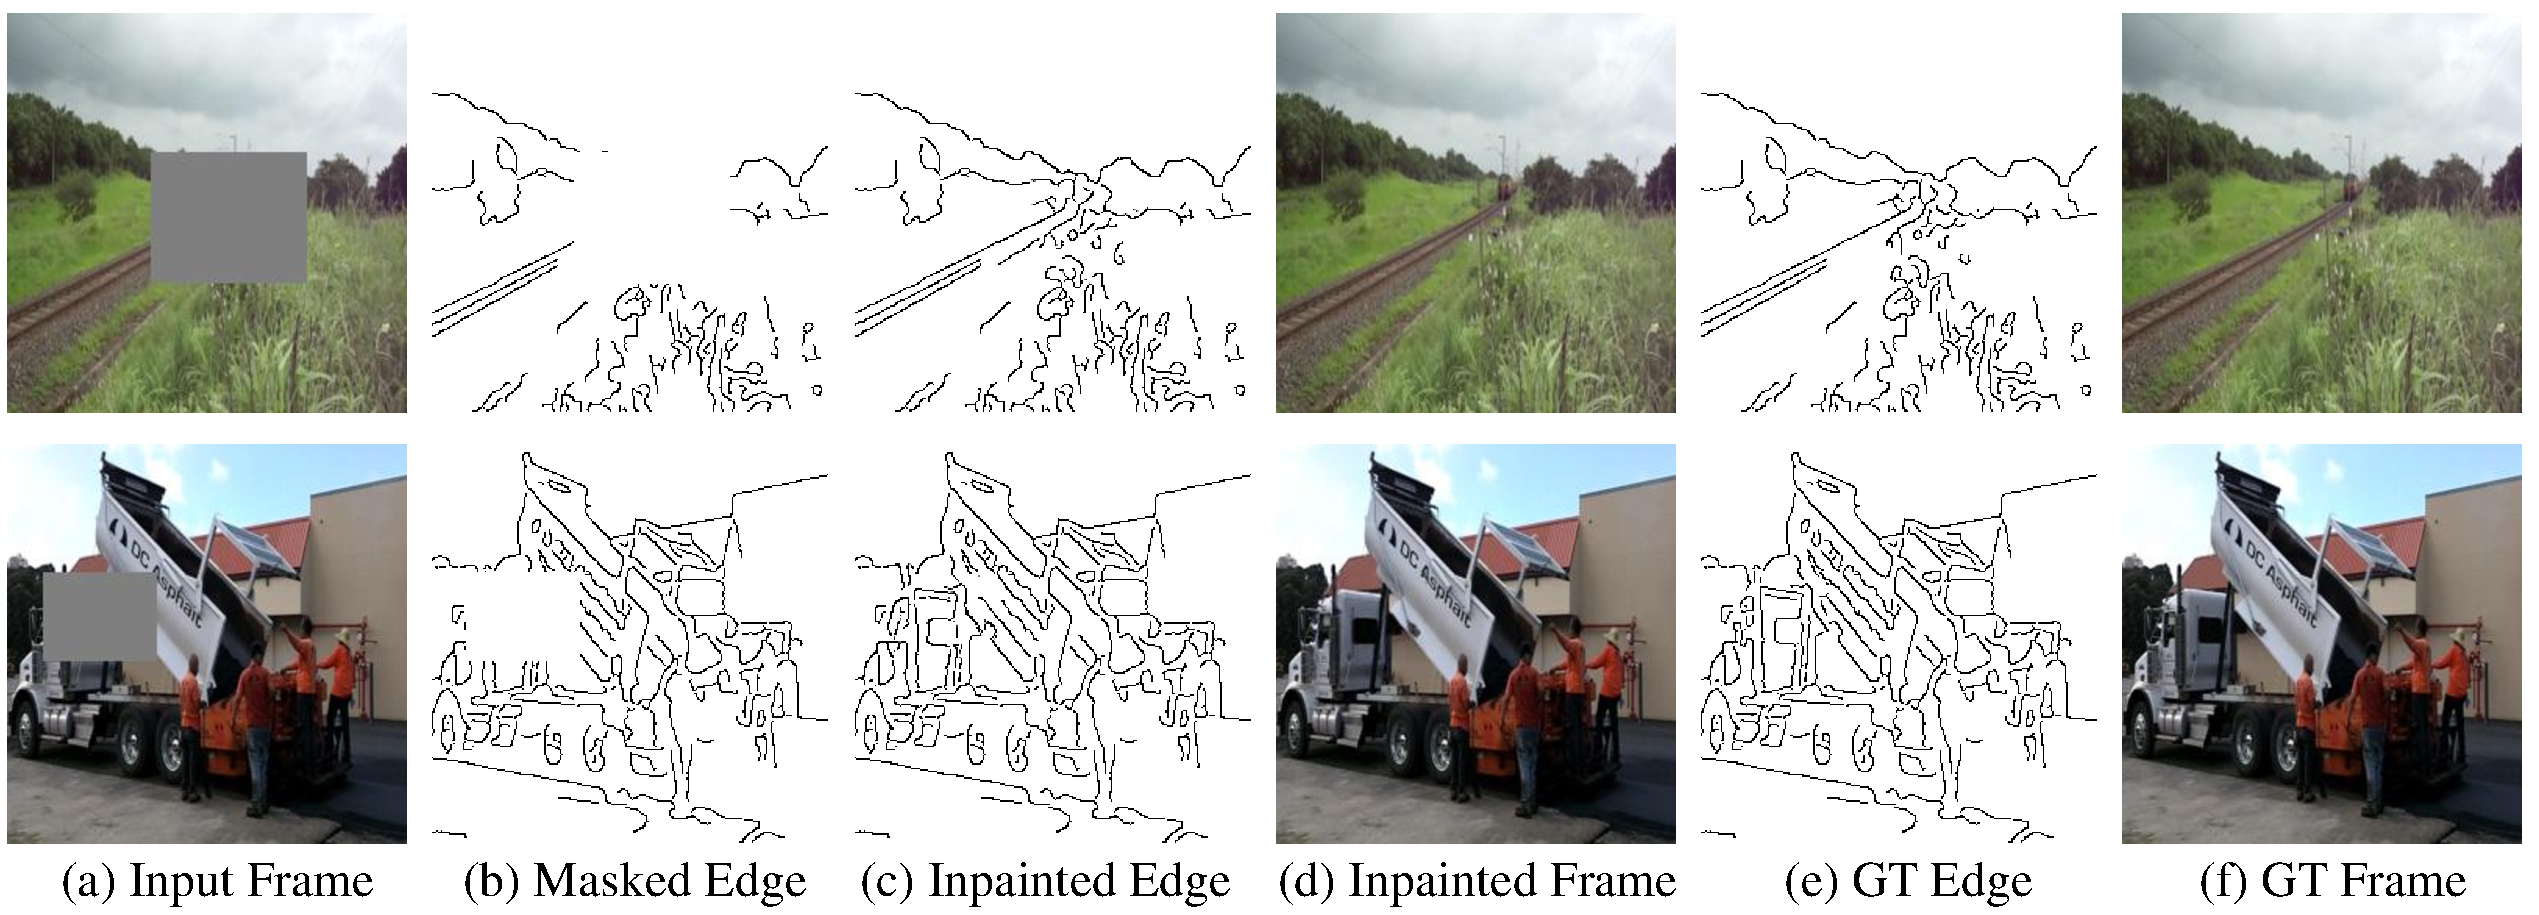
\includegraphics[width=0.97\columnwidth]{edgevis} % Reduce the figure size so that it is slightly narrower than the column. Don't use precise values for figure width.This setup will avoid overfull boxes. 
	\caption{Visualized effects of exploring structure edges in video inpainting. It's obvious that we can obtain more detail-clear results with structure guidance.}
	\label{edgevis}
\end{figure}




\begin{figure}[t]
	\centering
	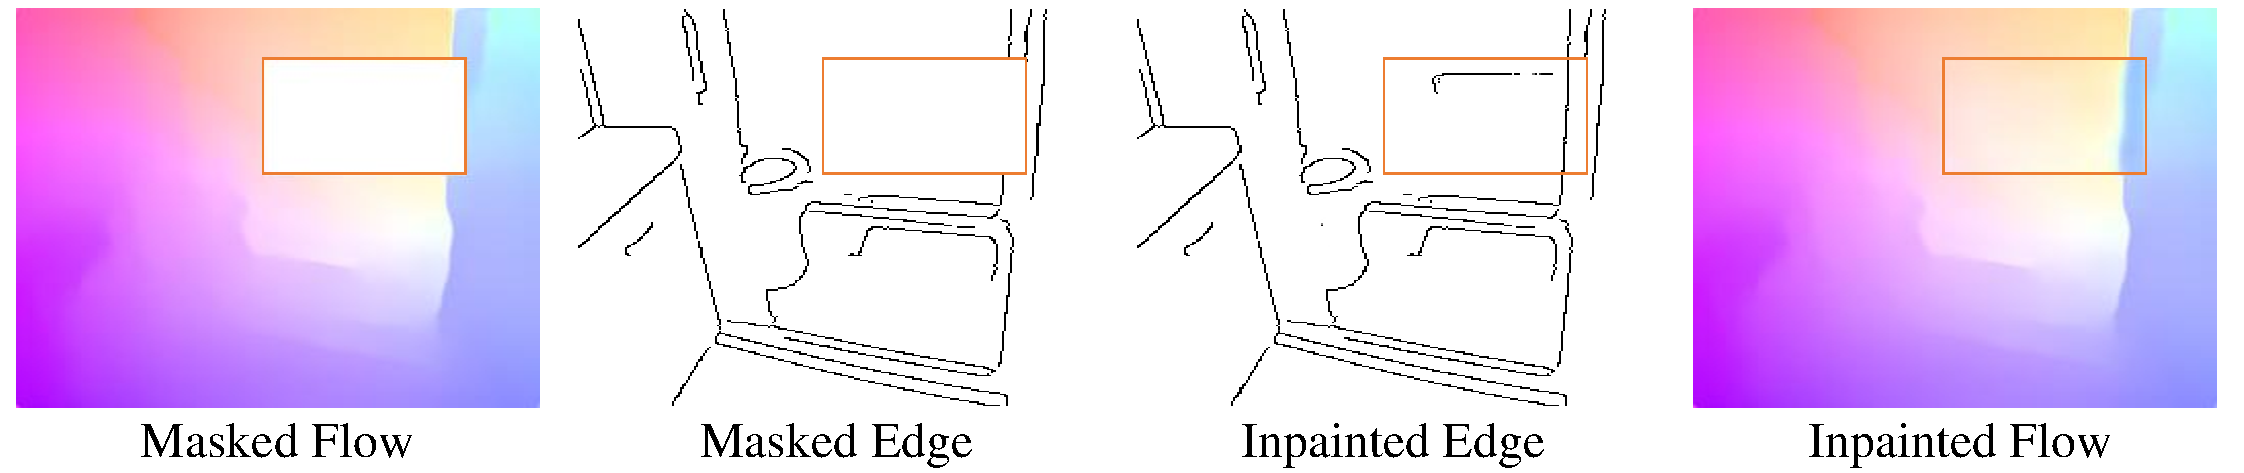
\includegraphics[width=1.0\columnwidth]{flowvis} % Reduce the figure size so that it is slightly narrower than the column. Don't use precise values for figure width.This setup will avoid overfull boxes. 
	\caption{Visualized optical flow predicted by our method.}
	\label{flowvis}
\end{figure}
\begin{figure}[t]
	\centering
	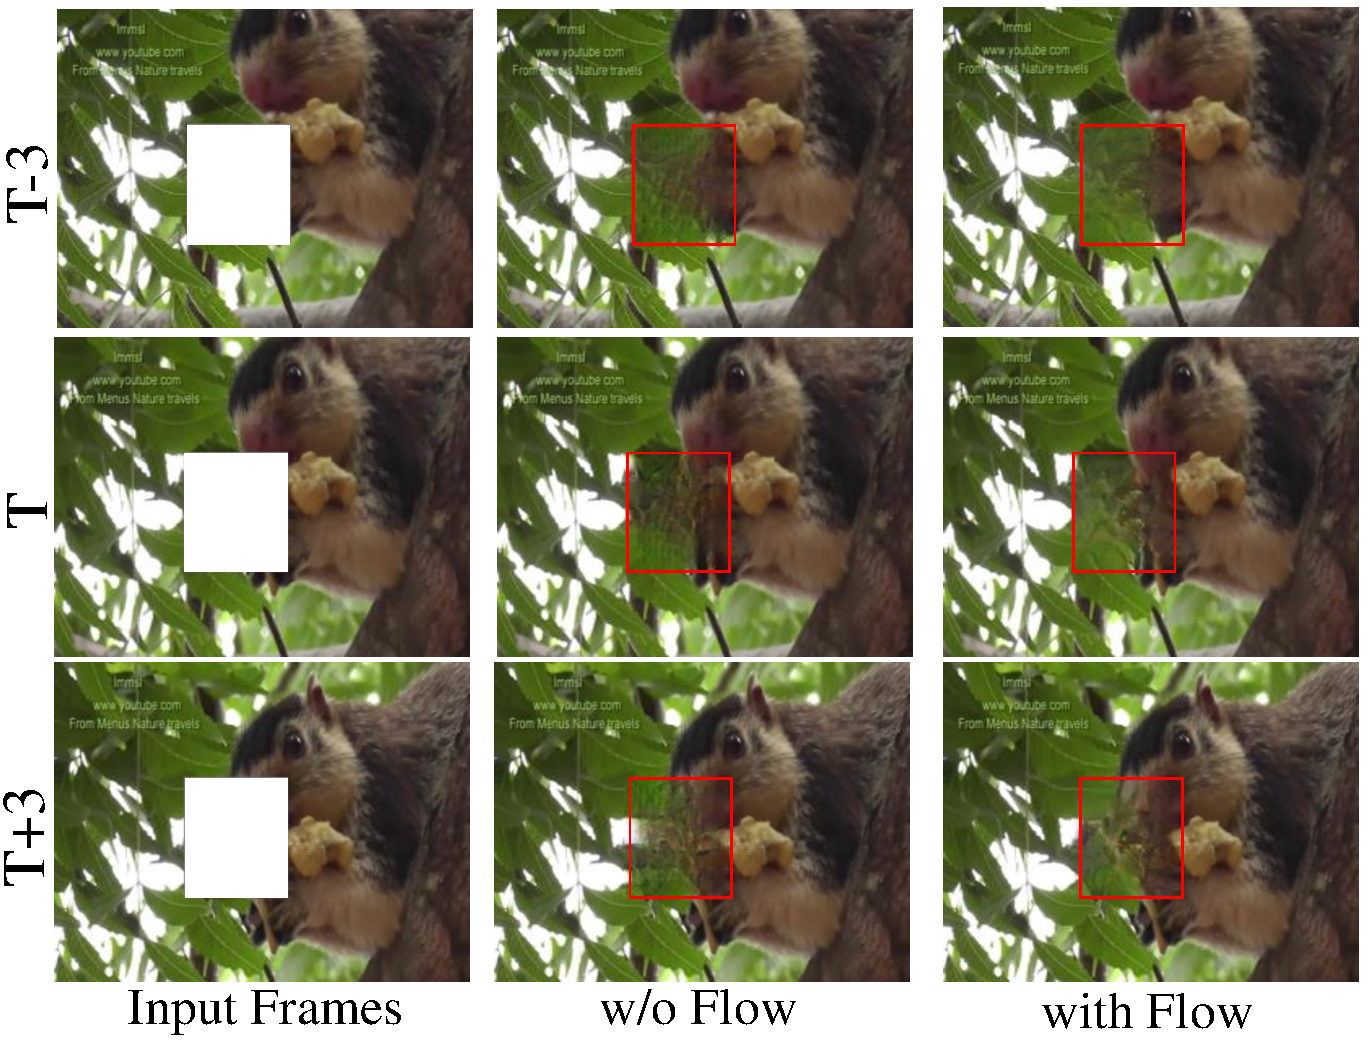
\includegraphics[width=1.0\columnwidth]{flow_vis} % Reduce the figure size so that it is slightly narrower than the column. Don't use precise values for figure width.This setup will avoid overfull boxes. 
	\caption{Visualized effects of temporal information.}
	\label{flow_vis}
\end{figure}

\subsubsection{Effect of Temporal Information in STINet.}
Temporal consistency is also an important factor in video inpainting. In our method, we utilize temporal information by flow-guided warping loss and temporal ensemble module to smoothen the artificial flickers and propagate complementary information from neighboring frames. 
%We use '+flow' to denotes the model 
Before temporal smoothing analysis, Fig.~\ref{flowvis} gives that visulized result, which proves that FNet can effectively complete the missing flows with fine boundaries.
The quantitative results are shown in Table~\ref{tab:sem}, We use 'Ours' to denote the model that apply flow information to '+SAM', which is the full model that we propose. It can be seen that the results is further improved after utilizing temporal information. The results prove that the complementary contents can be aggregated by motion, which is helpful in video inpainting. Surely the promotion brought by temporal information is not as much as that of structure information. However, the motion information can smoothen artificial flickers, resulting in temporal consistent inpainting results, which is shown in Fig.~\ref{flow_vis}. We can observe that the colors changes more in generated frames without flow. It also shows that the inpainted frames with flow can be more visually pleasing.  
%a flow warping loss to smoothen the artificial flickers and propagate complementary information from neighboring frames. 
 %It is achieved by $\mathcal{L}_{fec}$, which demonstrates that structure information can also boost the completion of optical flow.
%To evaluate the impact of temporal smoothening in STI, we compare two baselines, STI and STI w/o flow.
%As shown in Table~\ref{tab:edge}, STI works better than STI w/o flow, values...!!!.
%The visualized results are shown in Fig.~\ref{flow_vis}.
%It can be observed that the artificial flickers are alleviated when motion guidance is involved. 
Both the quantitative and qualitative results prove that the motion information is beneficial to temporal consistency as well as inpaitning.
%Besides, he visulization results in Fig.~\ref{flowvis} shows that $\mathcal{L}_{fec}$ encourages the network to predict optical flow  which demonstrates that structure information can also boost the completion of optical flow.

%We only use the first three mask settings on YoutubeVOS.
%\cxj{for what reason? page limit of the paper? How about others? Can we result in the same conclusion for different mask settings?}


%We discussed four variants of our method. We 
%\begin{enumerate}
%	\item STI: The Spatio-Temporal Inpainting network without guidance of either edge or flow.
%	\item +edge:
%	\item Free-from mask. We apply irregular mask which imitates hand-drawn masks on each frame, following \cite{liu2018partialinpainting}. 
%	\item Foreground object mask. This type of masks are defined to line out the foreground objects in videos, which is used for object removal.
%\end{enumerate}
%\noindent \textbf{Baselines.} Several variants of STSENet are defined as following. (1) STI w/o flow: The Spatio-Temporal Inpainting network without flow guidance \cxj{with or without EdgeNet and SEM?}. (2) STI w/o edge: The Spatio-Temporal Inpainting network without structure guidance. (3) STSENet w/o $\mathcal{L}_{fec}$: The Spatio-Temporal Inpainting network with guidance of both structure and motion, but $\mathcal{L}_{fec}$ is not used. (4) STSENet is the model which uses all modules proposed in this paper. 
%
%\cxj{We discussed four variants of our method. Use that version. }

\subsection{Comparisons with Existing Methods.}
We compare our results with state-of-the-art inpainting methods \cite{nazeri2019edgeconnect,wang2019video,Kim_2019_CVPR1,Xu_2019_CVPR}. 
As shown in Table~\ref{tab:sem}, Our structure-oriented method achieves better results than other methods with low time consumption, which demonstrates the effectiveness of utilizing both structural edges and optical flow in video inpainting. Notably, we can also get better results than existing methods when the optical flow is not added. The inference speed is almost twice faster. This indicates that structure clues can bring strong promotion to video inpainting, 
We also give qualitative results in Fig.~\ref{viszong}. Compared with existing methods, inpainting results predicted by our method are more realistic with finer details. We can observe that the frames prediceted by our method contain more sharper object contours.This is achieved by the effectiveness of structure information in video inpainting.















%\noindent \textbf{Effect of Flow-Edge Consistency Loss.}
%Flow-edge consistency loss $\mathcal{L}_{fec}$ is designed for mutual improvement of optical flow and edge maps.
%To demonstrate the effectiveness of $\mathcal{L}_{fec}$ in training, we compare the performances between STSENet w/o $\mathcal{L}_{fec}$ and STSENet. We use standard end-point-error (EPE) metric to evaluate the completion of optical flow. Besides, the well-completed flow and edge aid the final inpainting results, so the quality of final inpainting results also reflects the impact of $\mathcal{L}_{fec}$.
%The quantitative results are shown in Table~\ref{tab:lfec}. It indicates that $\mathcal{L}_{fec}$ plays a positive role in prediction of flow and edge, which is helpful for video inpainting. 
%\begin{table}[t]
%	\caption{The effect of structure clues and temporal smoothening in STSENet. The mask number denotes the indexes of mask setting in the section Experimental Settings. We compare STI,STI w/o SEM, and  in three aspects of metrics.}\smallskip
%	\centering
%	\resizebox{.95\columnwidth}{!}{
%		\smallskip\begin{tabular}{c|c|c|c|c|c|c|c|c|c }
%			\hline
%&\multicolumn{3}{c|}{Fixed Square}& \multicolumn{3}{c|}{Moving Square}&\multicolumn{3}{c}{Free-Form}\\
%\cline{2-10} 
%&PSNR & SSIM & FID & PSNR & SSIM & FID & PSNR & SSIM & FID\\
%\hline
%STI &28.0174 &0.9494  &  42.7164   &	
%33.8131 &  0.9705  &8.2390	& 
%30.0680& 0.9390 & 20.6358
%\\
%\hline
%+edge input  &29.5242 &  0.9520& 36.2097   &	
%37.6630	& 0.9798 &3.5161    &	
%33.8206	&0.9659  &    6.6651  \\
%\hline
%
%+SEM &29.9918 &  0.9533 &  27.4198  &	
%38.2433	& 0.9807 &   2.5083  &	
%35.7783	&0.9712  &   5.8786  \\
%\hline
%
%+flow &\textbf{30.0590} &\textbf{0.9543}&   \textbf{27.2431}  &
%\textbf{38.8186} & \textbf{0.9824} & \textbf{2.3455} &
%\textbf{35.9613}  & \textbf{0.9721}&  \textbf{ 5.8694} \\
%
%\hline
%			
%			
%		\end{tabular}
%	}
%	\label{tab:edge}
%\end{table}






\subsection{User Study on Video Object Removal}
Evaluation metrics can not fully reflect the quality of inpainted videos. So in addition to qualitative comparison, we also conduct a user study on DAVIS dataset to evaluate the visual quality of our method. We compare our method with the strong methods \cite{nazeri2019edgeconnect,wang2019video,Kim_2019_CVPR1,Xu_2019_CVPR}.
In each test, the origianl video, result produced by our method and result of another method are shown at the same time. The participants are allowed to play the videos multiple times to notice the differences of results of different methods.
we invite 30 participants for the user study. Each participant has to watch 20 random videos carefully, and choose which method is visually better. We list the preferred proportion of each methods compared to ours. The results are reported in Table~\ref{tab:userstudy}, which shows that our method is preferred by the users. Visualization in Fig.~\ref{vis_forg} also demonstrates that the results generated by our methods are visually better than existing methods.
\begin{table}[h]
	\caption{The result of user study.}\smallskip
	\tiny
	\centering
	\resizebox{0.7\columnwidth}{!}{
		\smallskip\begin{tabular}{c|c}
			\hline
			Comparing Methods&Preferred Proportion\\
			\hline
			Ours/Nazeri et al.&0.9083/0.0917\\
			\hline
			Ours/Wang et al. &0.8015/0.1985\\
			\hline
			Ours/Kim et al. b &0.7357/0.2643\\
			\hline
			Ours/Xu et al. &0.5941/0.4059\\
			\hline
			
			
		\end{tabular}
	}
	\label{tab:userstudy}
\end{table}


\begin{figure}[t]
	\centering
	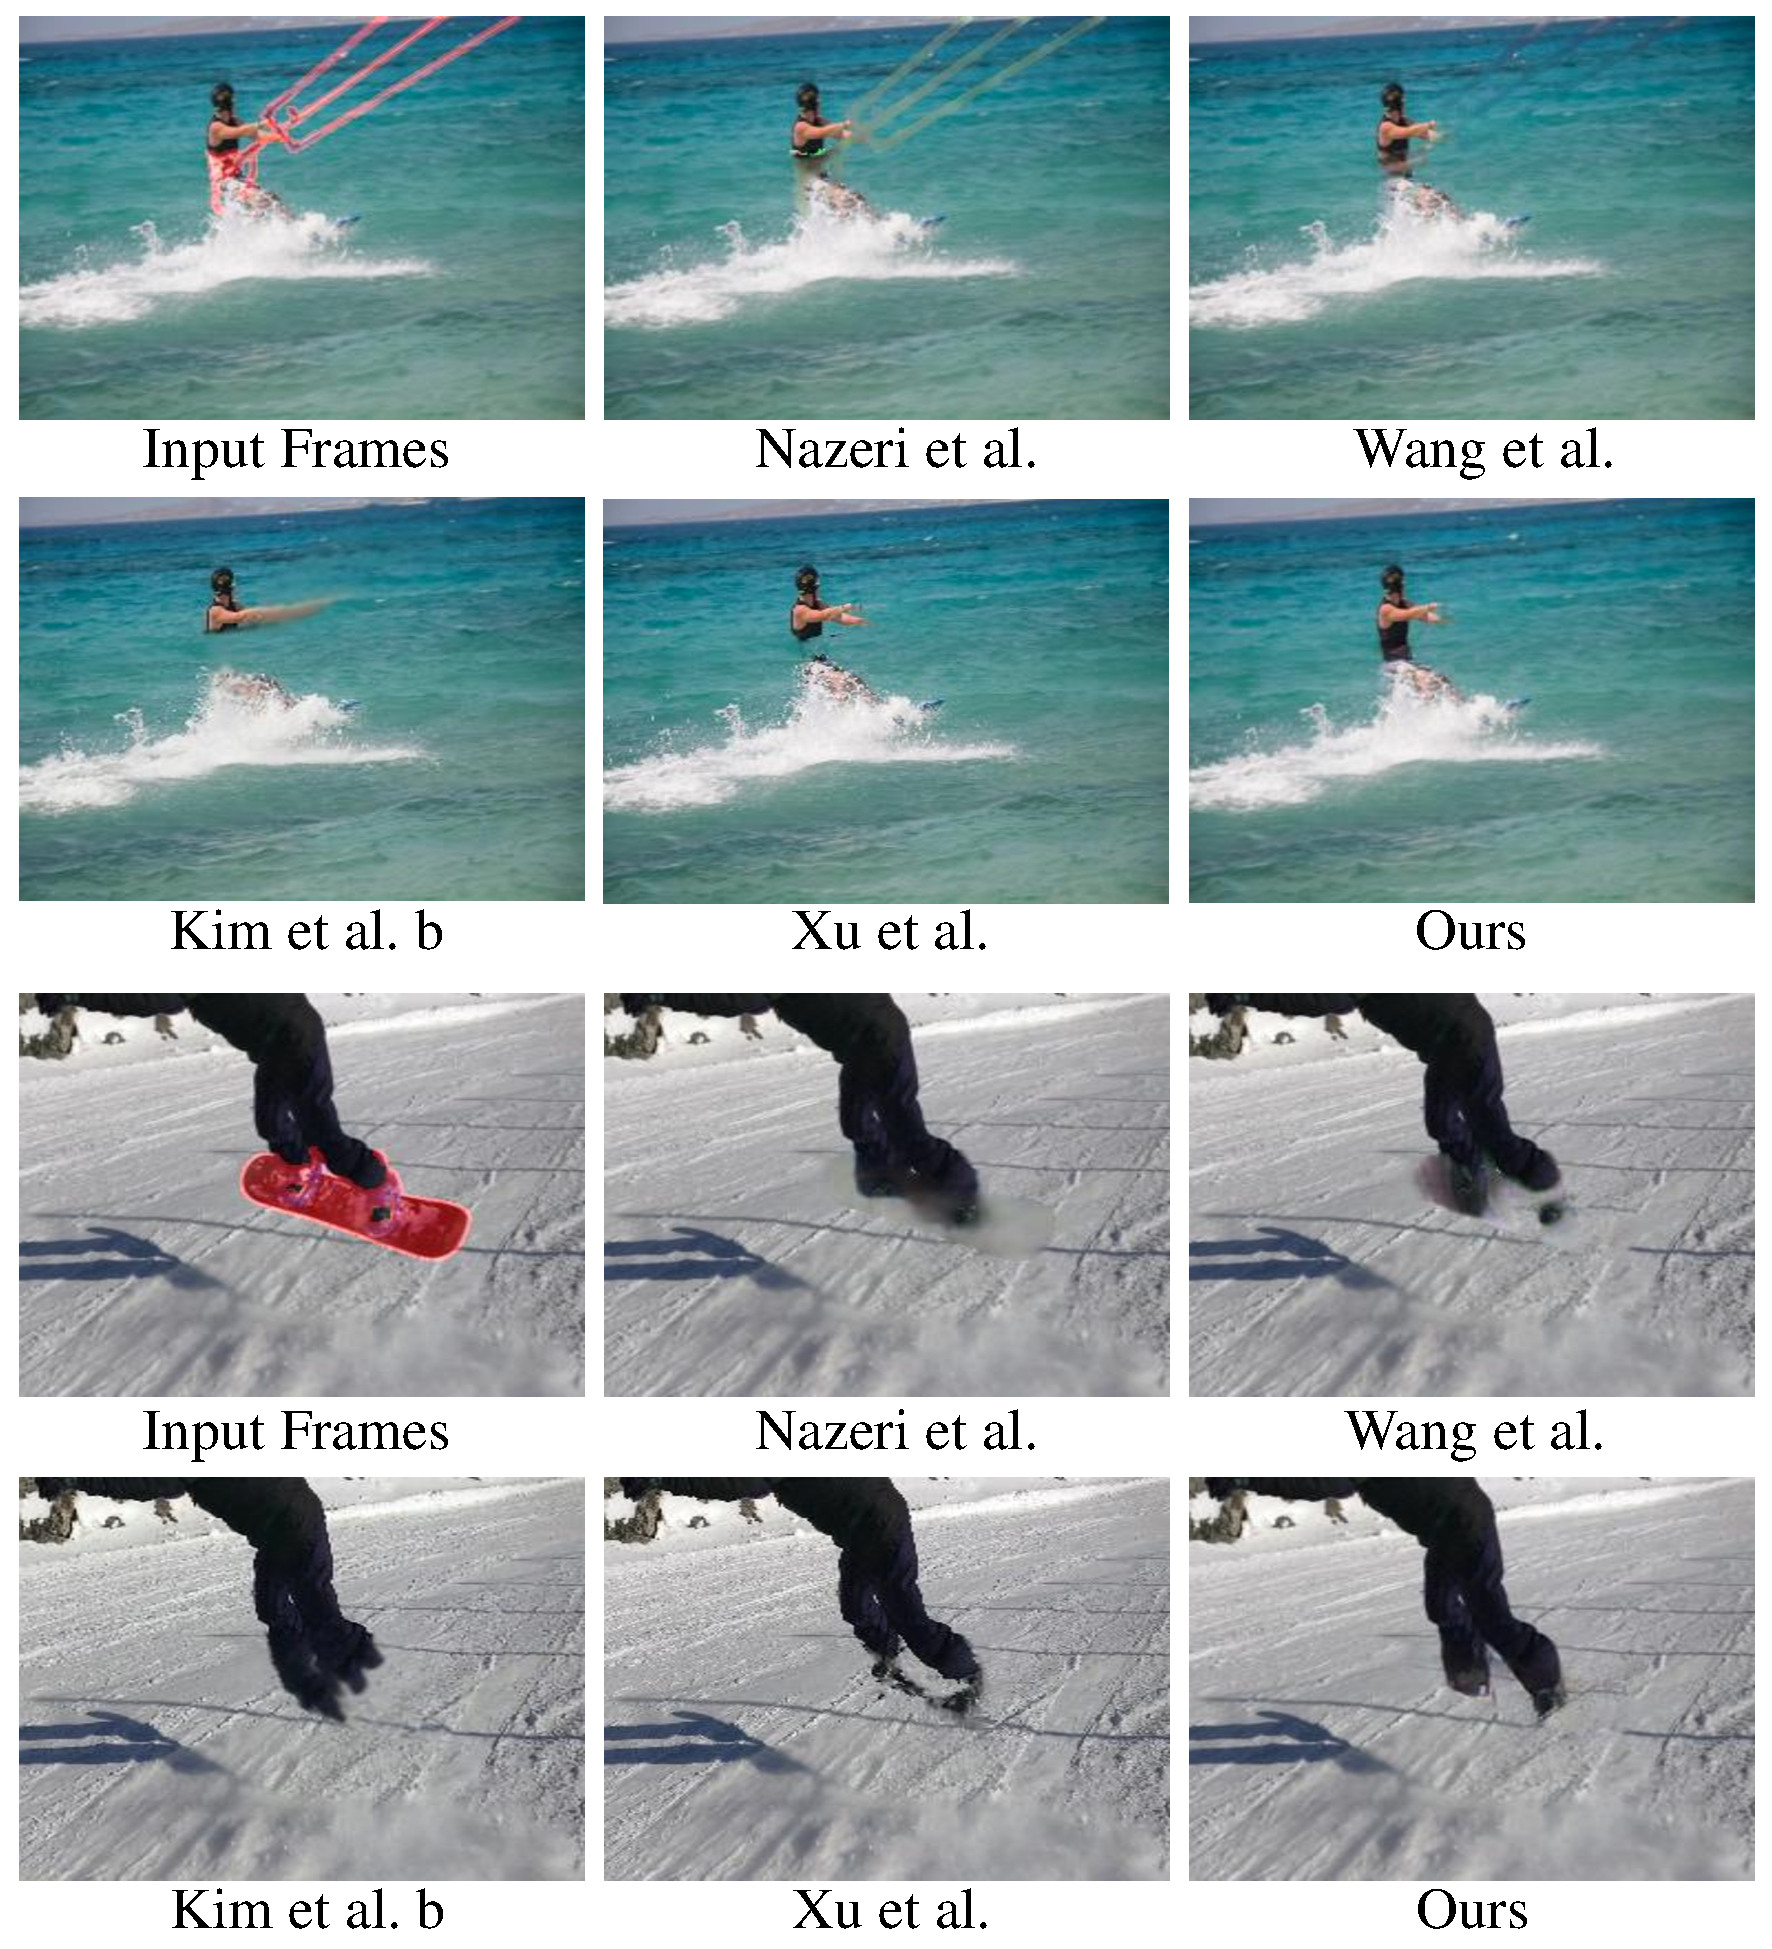
\includegraphics[width=1.0\columnwidth]{vis_forg} % Reduce the figure size so that it is slightly narrower than the column. Don't use precise values for figure width.This setup will avoid overfull boxes. 
	\caption{Visualized object foreground removal. The red mask in input frames indicates the object that we want to remove.}
	\label{vis_forg}
\end{figure}



\section{Conclusion}
In this paper, we propose a novel structure-oriented video inpainting method, which utilizes sturcture information to generate fine-detailed frames. We first complete edge maps, which indicate structure details in frames. Then we generate frames under the guidance of structure information. Besides, we synthesize missing optical flow to constrain the temporal consistency of final outputs.
Experiments on YouTubeVOS and DAVIS datasets demonstrate the effectiveness of our method of utilizing structure preserving in video inpainting.


% Specifically, we jointly complete edge maps and optical flow with a consistency loss, which helps to obtain temporal consistent edge and edge-clear optical flow. Then with the guidance of spatial details and motion tendency, spatio-temporal inpainting network is designed to predict the final video with fine spatial details few artificial flickers.
%The state-of-the-art performance on both YouTube-VOS and DAVIS prove the effectiveness of exploring structural clues and optical flow in video inpainting.
 
